\section{Introduction}
\label{sec:introduction}

\draftsuggestion{Extend the related-work coverage by searching for unit formation under segmentation, compression, patching, pooling, quantization, motif discovery, grammar induction, discretization, and state abstraction. Prioritize papers that introduce or directly evaluate tokenization. Retain reuse-only systems when they have broad impact, document a major public model, or supply a comparison that is missing from the review.}

\subsection{Motivation, Scope, and Contributions}

\draftsuggestion{State the intended readers, the inclusion rule, and the three contributions in terms that can be checked against the catalog. Keep examples representative rather than exhaustive. Present AI modality and domain object as two views of component tokenizers, then present complex systems as the composition of those components across modalities, objects, scales, or time.}

% Foundation models convert observed data into finite collections of model inputs. Language systems may use words, subwords, characters, or bytes. Vision systems may use pixels, patches, regions, or latent codes. Scientific models may use atoms, molecular fragments, residues, gene identifiers, mesh cells, or spectral peaks. The selected units determine what a model can address, compare, mask, predict, and allocate computation to.

% The literature does not use one name for this design choice. Relevant methods appear under segmentation, compression, patching, pooling, clustering, vector quantization, motif discovery, grammar induction, discretization, and state abstraction. We include a method when it constructs or selects finite addressable units for model input, output, intermediate computation, or reconstruction. This rule includes methods that do not use the word \emph{tokenization} but satisfy the definition in Section~\ref{sec:tokenizer-definition}.

% The review gives priority to papers that introduce a tokenizer, define one of its modules, or evaluate tokenization directly. We retain a system that only reuses an existing tokenizer when it provides an influential reference point, documents a major public model, or isolates a design choice that other retained papers do not test. This rule keeps the review focused while preserving evidence needed to compare tokenizers in practice.

% The scope covers symbolic sequences, images, video, audio, three dimensional geometry, graphs, tables, time series, fields, and spectra. Scientific sections study biological, chemical, physical, Earth, clinical, and embodied objects. A separate section examines systems that join modalities, objects, scales, or temporal states. The main object of analysis is a \term{tokenizer system} with training, encoding, and decoding modules. Section~\ref{sec:tokenizer-definition} states when a paper defines the full system and when it defines only one component.

% The paper makes three contributions. First, it gives a common mathematical definition for fixed alphabets, learned vocabularies, continuous units, and discrete neural codebooks. Second, it separates construction method, AI modality, domain object, and complex-system composition. Third, it defines evaluation controls that distinguish information retention, scientific validity, downstream utility, and compute cost.

\subsection{From Compression to Intelligence}

\draftsuggestion{Trace the technical line from coding and dictionary compression to subword learning, vector quantization, fixed patches, and learned unit selection. Emphasize which ideas changed tokenizer training, encoding, or decoding. Avoid presenting the history as a sequence of foundation-model architectures.}

% Tokenization links coding, compression, and statistical prediction. Information theory formalized the relation between symbol probabilities and code length \citep{shannon1948}. Later text systems learned reusable variable-length units from a corpus. Byte pair encoding (BPE) was adapted to open-vocabulary neural machine translation \citep{sennrich2016}. This example shows that the vocabulary and the segmentation rule are separate parts of a tokenizer.

% Vision and audio systems developed related choices. Vision Transformers expose fixed image patches as model units \citep{dosovitskiy2021vit}, while vector-quantized models learn discrete codes from continuous signals \citep{oord2017vqvae}. These examples separate three operations: forming boundaries, computing token values, and optionally mapping values to a finite codebook.

% Relational and scientific data study structures that a flat sequence does not represent directly. Graph tokenizers may use nodes, walks, or subgraphs. Molecular tokenizers may use string symbols, atoms, fragments, or grammar rules. Protein and cellular models may use residues, local structures, genes, or learned states. Across these cases, a token has limited meaning unless the representation also contains order, adjacency, geometry, or another relation.

% These systems share a common design pattern. A method chooses a base representation, forms units at one or more scales, stores relations, and defines what can be recovered. Its modules may be algorithmic, neural, or hybrid. Section~\ref{sec:tokenizer-systems} defines this pattern. Sections~\ref{sec:ai} and~\ref{sec:science} compare component tokenizers by AI modality and domain object. Section~\ref{sec:joint-systems} studies their composition in complex systems, and Section~\ref{sec:principles} states how competing choices can be tested.

\subsection{Observations and Insights}

\draftsuggestion{\textbf{Tokenizer systems are often compared only through their output units.} Test whether reported conclusions change after separating tokenizer training, encoding, and decoding. Useful cases include subword vocabularies with different segmentation rules, visual codebooks with different decoders, and molecular vocabularies with incomplete inverse mappings. Keep this observation provisional until each case has direct evidence.}

\draftsuggestion{\textbf{Scientific token identity often depends on relations and scale.} Compare atoms with motifs, residues with structure units, genes with cell states, and grid cells with adaptive regions. Record when geometry, symmetry, experimental condition, or task changes the useful unit. Include cases where fixed small units remain the stronger choice.}

\draftsuggestion{\textbf{Compression, reconstruction, and scientific utility can disagree.} Look for tokenizers that reduce sequence length or reconstruction error while losing rare events, valid composition, intervention response, or transfer information. Compare the tokenizer training objective with every later evaluation target before making a general claim.}

\begin{figure}[t]
    \centering
    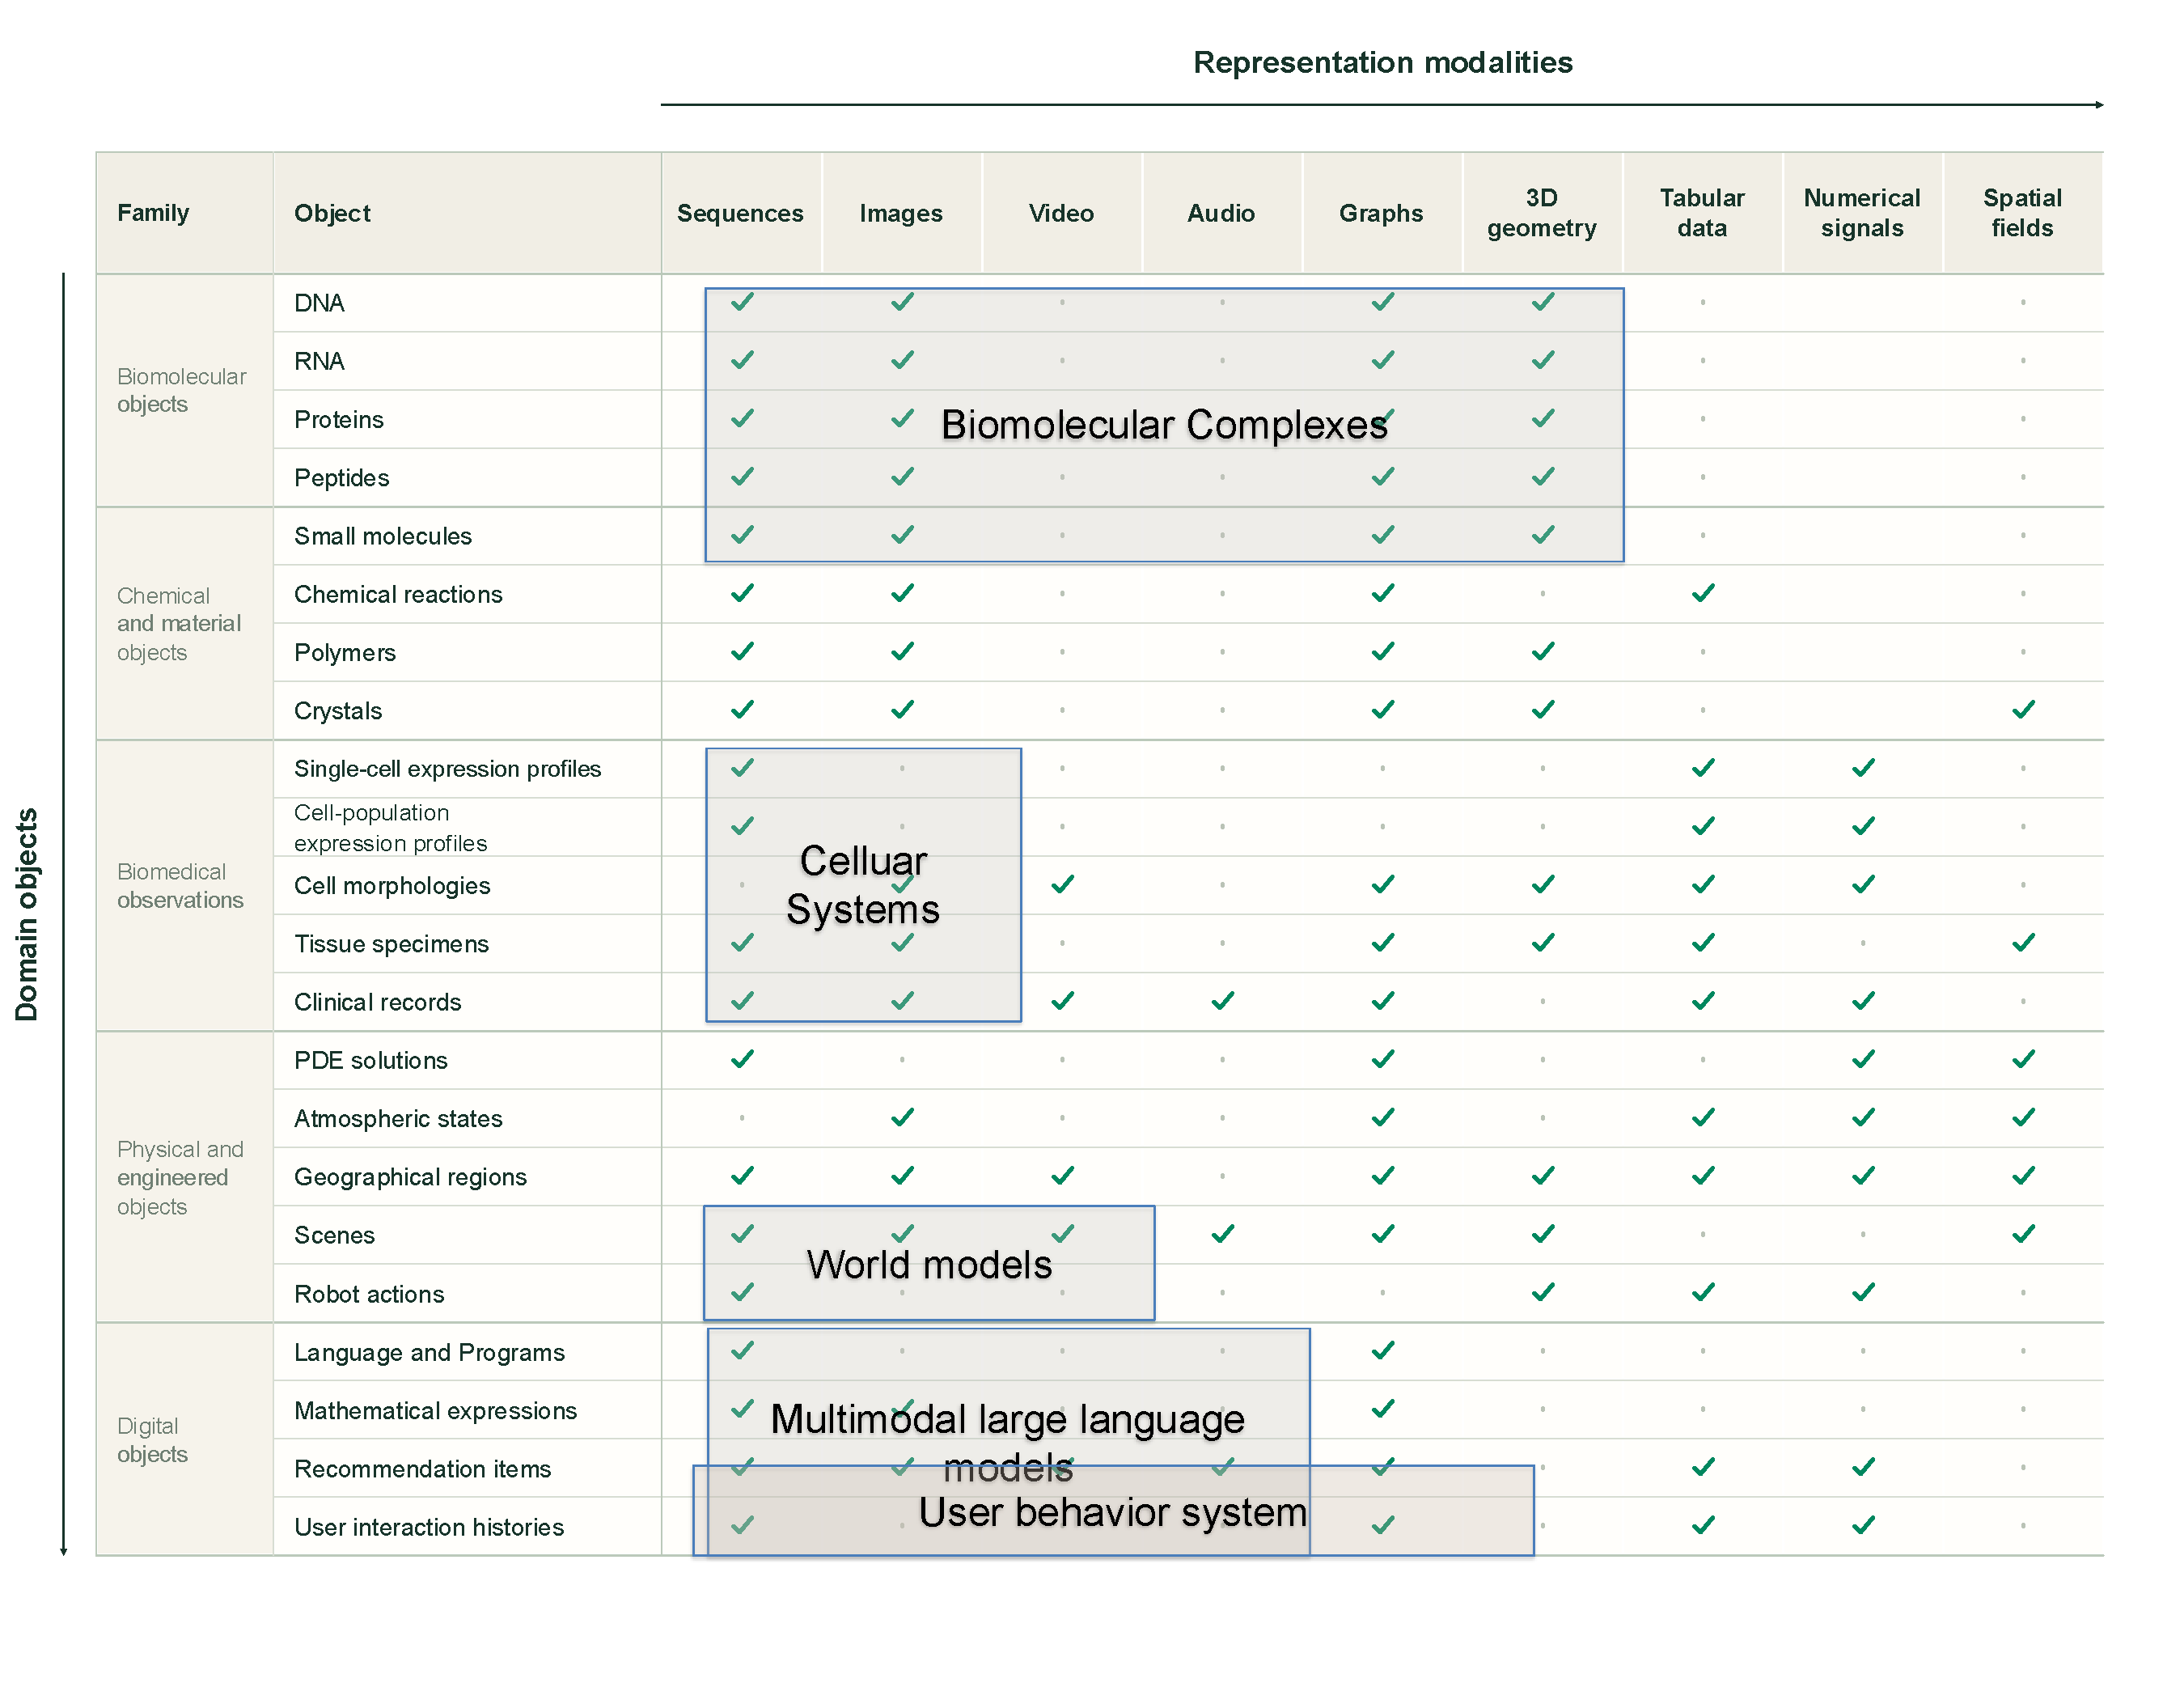
\includegraphics[width=\linewidth]{figures/overview.pdf}
    \caption{Overview of the work: We organize the review into two major dimensions (representations and objects). (The current tick is tentative; feel free to let me know your suggestion and to remove or add new ticks based on your survey.)}
    \label{fig:overview}
\end{figure}